% !Mode:: "TeX:UTF-8" 



\BiSection{2.3}{Figures}

\fancyhead[R]{本题2.3由QC.Z完成}

导出用$I_{D}$和 $\frac{W}{L}$表示的$g_mr_o$的表达式。画出以L为参数的$g_mr_o \sim I_{D}$的曲线。注意$\lambda \propto \frac{1}{L}$。

解:

$g_m=\sqrt{2\mu_nC_{ox}\frac{W}{L}I_D}$

$r_o=\frac{1}{\lambda I_D}=\frac{1}{\frac{1}{L} \times I_D}=\frac{L}{I_D}$

本征增益$A=g_mr_o=\sqrt{2\mu_nC_{ox}\frac{W}{L}I_D} \times \frac{L}{I_D}=\sqrt{2\mu_nC_{ox}\frac{WL}{I_D}}=K\sqrt{\frac{WL}{I_D}}$,常量$k=2\mu_nC_{ox}$

$A \propto \sqrt{L}\sqrt{\frac{1}{I_D}}$

当$L=L_1=1,I_D=2 \text{时}A \propto \sqrt{\frac{1}{2}}=0.707$

当$L=L_2=2,I_D=2 \text{时}A \propto \sqrt{\frac{2}{2}}=1$

当$L=L_3=3,I_D=2 \text{时}A \propto \sqrt{\frac{3}{2}}=1.225$

		\begin{figure}[H] %H为当前位置,!htb为忽略美学标准,htbp为浮动图形
	\begin{minipage}{\linewidth}
		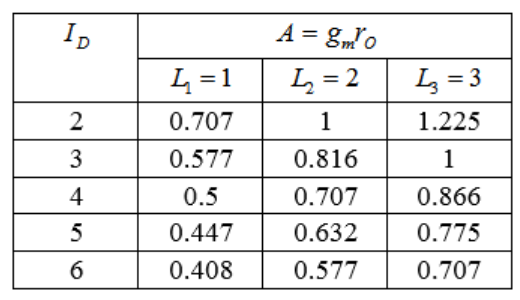
\includegraphics{2.3-1}
	\end{minipage}
		\caption*{图1} %最终文档中希望显示的图片标题
\end{figure}

\begin{figure}[H] %H为当前位置,!htb为忽略美学标准,htbp为浮动图形
	\begin{minipage}{\linewidth}
		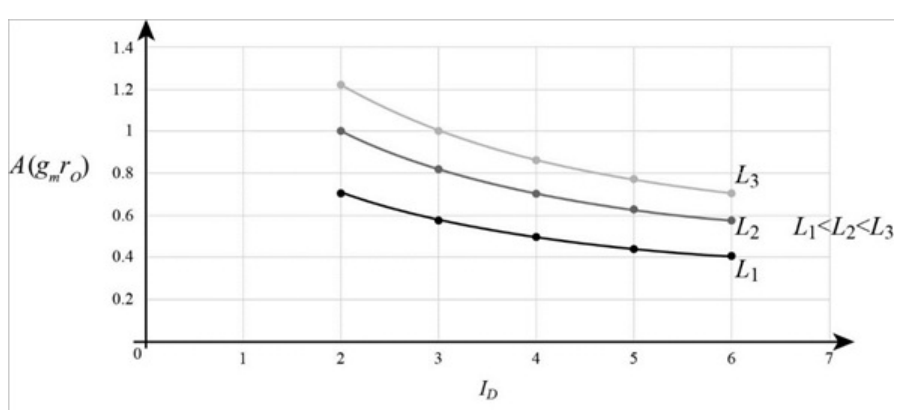
\includegraphics{2.3-2}
	\end{minipage}
		\caption*{表1} %最终文档中希望显示的图片标题
\end{figure}